%! Suppress = MissingImport
\section{Waterfall Methodology}\label{sec:waterfall-methodology}
%https://en.wikipedia.org/wiki/Waterfall_model#History
The waterfall methodology was first introduced in the 1950's by Mr.
Benington but was only formalized in 1970 by  Winston W. Royce.
This methodology has been widely used in the industry, although it received
a lot of criticism few decades after.

This section will first present the key concepts of this methodology followed
by the detailed workflow.
After that, we'll point out its weaknesses and present a improved version:
the V-model.
Finally, we'll state the residual problems and limits of the improved model.

\subsection{Key concepts}\label{subsec:key-concepts}

The two main phases in software development are \textit{Analysis} and
\textit{Coding}.
Even projects with no clear methodology will at least go throw those two phases
that define and build the software.
However, these steps are only the emerged part of the iceberg.
Any software will require some specific design regarding its architecture, the
technologies it will use, its production environment and will also need time
to verify that the software actually works.

\begin{figure}
    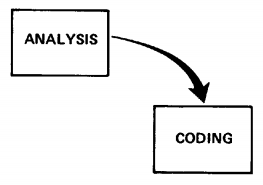
\includegraphics{../../images/waterfall/analysis_coding.PNG}
    \centering
\end{figure}

The problem stated by Royce is that these design and testing steps were not very
well regarded, simply because they didn't directly add any business value.
Therefore, these steps were not very valuable from a client point of view and
were likely to be skipped. \\
Ignoring these steps often leads to horrific and costly overrun.
For example, fixing an architectural issue in a software might require a
complete new design and the developers will have to start all over again.
Also a lot of bugs will only be uncovered in production because of a lack
of testing effort, in terms of both strategy and execution.
New versions of the software will have to be made in order to fix them, while
hoping not adding new problems.

Royce then proposed a model that adds extra steps to the development process,
to better design the software before implementing and better test it before
releasing it.

We'll see more details later about the workflow itself.
The main improvement is that we now have more design steps, a dedicated step
for testing and also one for the operations phase.
These steps that aren't directly related to the business value of the
software are now part of the nominal development process.

%TODO remove this figure as we do not describe the steps in the workflow ?
\begin{figure}
    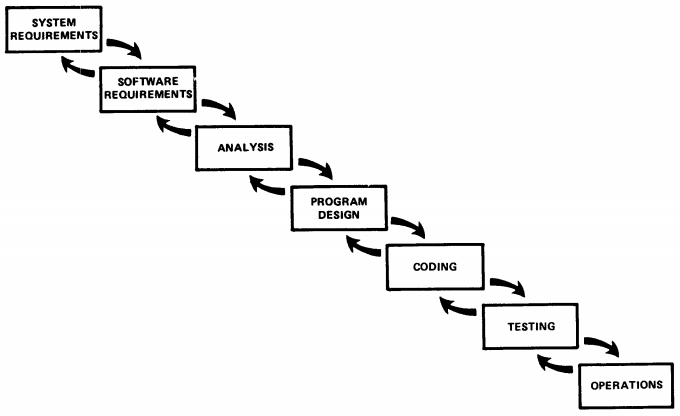
\includegraphics[width=\textwidth]{../../images/waterfall/waterfall.PNG}
    \centering
\end{figure}

\subsubsection{Documentation}

This emphasis on the design of the software makes the waterfall very
document-oriented.
This is one of the main traits of this methodology and there're a several
types of documents:
Software requirements, preliminary program design, interface design, final
program design, test plan and operations instructions.
These documents will help in several ways the project.

The formal aspect of written documents are nice during the design
specification by providing a tangible evidence of the understanding of a
requirement or the definition of a program interface.
A misunderstanding can easily be detected during a read over phase, by the
author, the analysts and the client.
This also prevent the project from forgetting a feature or any detail mentioned
during an informal meeting.

The documentation externalizes the knowledge from the analysts and clients
minds, which will benefit the whole project team.
Future maintainers of the application won't have to dig into the code base to
understand what it does, they will simply have to look at the structured
documentation to do so.

The operations phase will also take advantage of a well documented
application.
Installation or deployment processes will be clearly defined and even people
that  weren't there during the development phase will be able to start and
run the program.

\subsubsection{Testing}

The waterfall methodology also puts testing a bit more at upfront, by adding
it as a required step in the development process.

As we mentioned it in the previous section, this methodology is very
document-oriented and this becomes very handy for the testing phase.
The documentation provides a comprehensive overview of all the requirements
and features of the application, this will greatly help for the test
strategy.

The strategy will drive the design of test cases and also define the
required data set to execute them.
This test plan is very important and is made even before the implementation
phase, to ensure that the validation of the final product is doable.

Once the strategy is done, the test cases redaction can be started at any
time, whether before, after or in parallel of the implementation phase.
This let the time to the test team to nicely prepare the test phase.

\textit{Documentation} and \textit{Testing} are really the two new main
concepts of the waterfall methodology.
The documentation helps to structure the software development process and
makes easier to write and execute.

\subsection{Workflow}\label{subsec:workflow}

This section is going to describe the workflow of the waterfall methodology.
Going from the design phases to the release, it'll cover how the
different teams work in each phase.
Some steps have been grouped into to a single sub section to make the
workflow smoother.

%https://www.guru99.com/hp-alm-introduction.html
The workflow will be illustrated with the use of an Application
Lifecycle Management tool.
An ALM tool is here too help the end-to-end management of a software project,
from the design to delivery.
All the requirements, specifications, test plans etc.
are centralized in this kind of tool.

\begin{figure}
    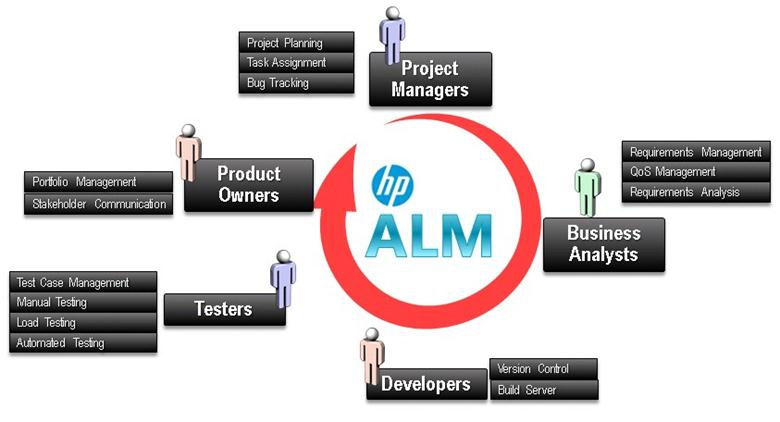
\includegraphics[width=\textwidth]{../../images/waterfall/alm_workflow.jpg}
\end{figure}

\subsubsection{Design phase}
The design phase is the first and most important in waterfall.
This phase can be decomposed into several steps: gather the customer
needs, define the requirements and design the solution.
Let's dig into each step.

The gathering of the customer needs is the first step of the design phase.
This is where the client presents its high level business needs to the
analysts and architects.
This can be done through workshops, meetings, presentations etc.
The commonly used supports are word documents or slides.

Once the analysts and architects have a clear understanding of the customer
needs, they will propose an architecture and the requirements.
Even if the solution isn't fully defined yet, the global architecture should be
able to fulfil all the requirements.

The requirements can be seen as a low-level representation of the customer
needs.
They are written by the analysts, validated by the client and managed using
the ALM tool, in order to keep them organized, centralized and formalized.

When the proposed architecture and requirements are validated by the client,
the specification of the solution can start.
In this phase, each requirement is analyzed and declined into a sub set of
specifications that will satisfy it.
These specifications can be either functional or non-functional.
The difference between the two is that a functional specification will
describe how the system should \textit{behave}, where the non functional will
define \textit{how} to do it.

All specifications will also be stored in the ALM tool and be mapped to
the requirements they cover.
One great advantage of an ALM tool is to compute the coverage of the
specifications.
We can see at a glance if there is a requirement that is not associated to at
least one specification.
This will prevent us from forgetting a requirement during the specification
phase.

\subsubsection{Test Strategy}
This step can be done by the analysts that wrote the specification or could be
handled by a complete external team, made of dedicated professional testers.
Thanks to all the documentation written in the design phases and the ALM tool,
it's indeed possible to externalize the testing phases and the project will be
able to leverage the experience of these professional testers.

During the test strategy, every specification is analyzed to determine which
acceptance test suite must be run in order to validate the feature.
The global workflow, dataset, environment setup etc.
Everything is planed before to make sure that the actual software design and
architecture can be validated in the end.

The ALM tool is again very useful because it allows to compute the coverage
of our specifications.
It's the same principle as the previous section, it simply checks if every
requirement as at least one associated test.
The coverage however can sometime be misleading because it may be complex to
represent every possible path for every requirement.
Therefore a requirement can be covered by a test, but in fact there's only one
nominal test case.
The others rare, but possible, paths are in fact not tested yet.

\subsubsection{Implementation}
The implementation phase starts once both the specifications  and
the test strategy are written.
A workshop is usually organized between the analysts and the dev team to
introduce them the business domain and the design of the global solution.

The technical leader will read the specifications and create sub tasks to
implement them.
An estimation of the time to implement it is made for each task and they are
then assigned to the developers.

The developer works on his local workstation and will commit is work to the
Version Control System (Git or SVN for example).
The team can commit its work on the same branch, following the process of
\textit{Continuous Integration} that will detail later.

Once the implementation phase is completed, some preliminary checks must be
done by the developers, like visual inspection by a peer or code reviews.
A certain amount of bugs can therefore be immediately fixed at a very low cost.
Also the team can learn from its mistakes and shouldn't do the same mistakes
next time.

The features should also be manually tested by the developers, before the real
testers do it.
This can be called \textit{Smoke tests}, their goal is to quickly test the
system to see if it \textit{looks like} working.
It's not an exhaustive testing phase, it simply avoids to deliver a software
that will explode after two tests.

\subsubsection{Testing phase}
The testing phase is decomposed in two phases, the test cases writing and the
their execution.
The writing can be done either before, after or during the implementation
phase, thanks to the already written documentation, both the dev and test
team can work in parallel.

A test plan, which simply represents all the test cases, is stored in the ALM
tool.
Therefore we can keep each test plan, for each version of the software.
We can also access to the coverage of the test plan regarding the
specifications and requirements.

The test plan can also be executed using the ALM tool.
Each test case can be started by a tester, that will do the action specified in
each test step.
He will then compare the expected result vs the actual result and add a proof
of validation (like a screenshot or log files).
When the actual result is wrong, a new defect will be raised with a detailed
description of the error.

Once the test plan is completely executed, all the defects are collected and
analyzed.
The dev team will receive the list of the bugs to fix and will start over a
new dev phase and deliver a new release candidate.
This round trip between the dev and test team will occur while new defects
are uncovered.
Sometimes, because of delivery deadlines, minor defects will be kept if there
is no major defect.

After this testing phase, the release candidate is now validated and becomes
the final release version of the software.

\subsection{Limits}\label{subsec:limits}
The waterfall model as it is, has some limits in practice and this section is
going to highlight the main one, that the V-model tries to solve.
The rest of the limits, shared between the waterfall and the V-model will be
mentioned later.

We've seen that the waterfall improved a classic development process by
adding extra design steps and a testing phase.
This testing phase is now mandatory and ensure that the released software is
working correctly.
When bugs are detected during this phase, new defects are created and sent to
the dev team.
This makes a costly round trip, in terms of time and therefore money.

The code of a software rarely works the first time, so the first round trip
raises a lot of defects.
Sometimes, a defect is tagged as \textit{blocking}, which means that some other
test cases cannot even be executed because of this bug.
The dev team need to fix it immediately and the whole test campaign must be
started over from scratch.

The problem comes from the abrupt transition between the implementation phase
and the testing phase.
Except the visual inspection and code reviews, there is no real test made by
the developers.
Hence the software is sent to the test team when it \textit{looks like}
working and it's likely to contains a lot of bugs.

Bugs must be detected as earlier as possible, even before the
testing phase and therefore by the developers.
This where the V-model improves the waterfall model, so we're going to
present it.

\subsection{V-Model}\label{subsec:v-model}
The V-Model is a improvement of the waterfall methodology and emphasis a
two key concepts: \textit{Verification and Validation}.
\begin{description}
    %https://www.softwaretestinghelp.com/what-is-stlc-v-model/
    \item[Verification:] Verification is a static analysis technique.
    In this technique testing is done without executing the code. \\
    Examples include - Reviews, Inspection and walkthrough.
    \item[Validation:] Validation is a dynamic analysis technique where
    testing is done by executing the code. \\
    Examples include functional and non-functional testing techniques.
\end{description}

Although these concepts were also present in the waterfall methodology, they
were not at the forefront of the development process.
Verification occurred at the end of the implementation phase, where the
developers would do code reviews and visual checks.
The validation part was during the testing phase, where the test cases
would validate the implementation of the specifications.

In the V-model, verification and validation occurs much more frequently,
even before the testing phase.
This last has also been extended and now occupies almost the half of the
development process.

\begin{figure}
    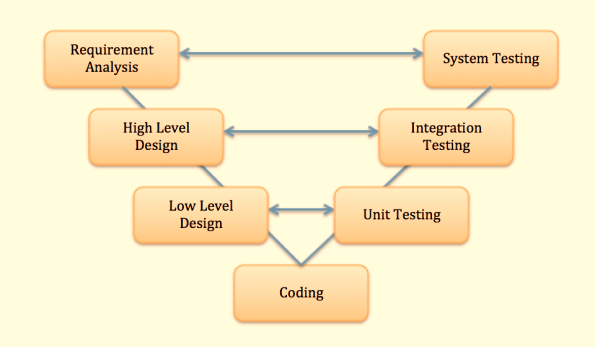
\includegraphics[width=\textwidth]{../../images/waterfall/v_model.png}
    % TODO fix position
\end{figure}

Two new kinds of tests are introduced, \textit{Unit} and \textit{Integration}
tests.

\subsubsection{Unit testing}
Unit tests are at a very low level and only verify  a method, component or
service alone, without its dependencies or external environment.
The System Under Test (SUT) is completely isolated and tested against specific
input and output.
This kind of tests asserts that the component works correctly, at least when
he's alone in a fake environment.

Tools such as \textit{Mockito} (and similar libraries) are very useful for
unit testing.
They allow to control the external services the component might need to
correctly be tested, like a database or a web service.

\subsubsection{Integration testing}
Integration tests are at a higher level and will test a component in a real
environment.
The other modules shouldn't be mocked, so the interactions between the SUT
and its environment are also verified.
Sometimes, modules are not yet developed or are not accessible from the
integration environment.
In this situation, mocking is allowed and should be as close as possible to the
real service.

Integration tests are a bit more difficult to write, because you need to have
all your other modules working correctly to not distort the test of the SUT\@.
These tests also usually require a bunch of data in the database or from some
web services, therefore a dataset must generated before the integration test.

In common web application framework, test utility libraries are provided to
easily set up an environment for integration testing.
When it's not provided, it requires to make a custom environment and can
quickly become costly to maintain.

\subsection{Residual limits}\label{subsec:residual-limits}
Now that we've covered the waterfall methodology and its improved version, the
V-model, we are going to list the residual problems of our development
process.
We'll see the limitations of the V-model in term of testing and also some
issues with the current document-oriented approach.

\subsubsection{Testing in V-model}
The V-model has significantly improved the waterfall methodology by adding
new kinds of test, in order to detect the bugs as soon as possible, using
Unit and Integration tests.
However, these tests have still one major issue, they always come after the
implementation phase.

When the code of a feature is written, the developer will write a unit test
for it.
He will have a fresh idea of the code he just written, therefore he will
usually go very straight forward.
He'll look at his code, see what are the expected parameters, the possible path
of the if/else blocks and the return values.
He will then write some assertions against the return values, like for example
verifying that the setters have been called with the right values.
He may also use a code coverage tool to see if all the lines of code are
covered.

The problem is that a test written with this approach is completely distorted
because it will only validate what have been written, and not necessarily
what should have been written.
The test is adapted to work with the existing code, which means that it will
validated the possibly already written bugs.
If the developer has missed a logical path or an attribute to modify from the
specification, the test won't check for it either.

These potential bugs will only be covered by tests that were written against the
specification, therefore only in the functional test phase which comes a bit
late in the development process.
So even if we can now detect some technical bugs thanks to the unit and
integration tests, they're not very useful to detect real bugs.

\subsubsection{Manual functional testing}
% TODO human errors are accepted but not fixed
% TODO automation is an optional step and usually a side task made by QA
% TODO the fear of having to re execute a test case again
% TODO already passed / unrelated test are not executed again

\subsubsection{Documentation limits}
% TODO too many locations
% TODO need a constant effort to maintain up-to-date all the sources
% TODO dev and analysts are separated
% TODO both the dev and analysts interpret alone the specifications
% TODO a lot of possible human error: spec, code, test cases writing and exec
% TODO human errors are accepted but not fixed
